%% bare_jrnl_compsoc.tex
%% V1.4a
%% 2014/09/17
%% by Michael Shell
%% See:
%% http://www.michaelshell.org/
%% for current contact information.
%%
%% This is a skeleton file demonstrating the use of IEEEtran.cls
%% (requires IEEEtran.cls version 1.8a or later) with an IEEE
%% Computer Society journal paper.
%%
%% Support sites:
%% http://www.michaelshell.org/tex/ieeetran/
%% http://www.ctan.org/tex-archive/macros/latex/contrib/IEEEtran/
%% and
%% http://www.ieee.org/

%%*************************************************************************
%% Legal Notice:
%% This code is offered as-is without any warranty either expressed or
%% implied; without even the implied warranty of MERCHANTABILITY or
%% FITNESS FOR A PARTICULAR PURPOSE! 
%% User assumes all risk.
%% In no event shall IEEE or any contributor to this code be liable for
%% any damages or losses, including, but not limited to, incidental,
%% consequential, or any other damages, resulting from the use or misuse
%% of any information contained here.
%%
%% All comments are the opinions of their respective authors and are not
%% necessarily endorsed by the IEEE.
%%
%% This work is distributed under the LaTeX Project Public License (LPPL)
%% ( http://www.latex-project.org/ ) version 1.3, and may be freely used,
%% distributed and modified. A copy of the LPPL, version 1.3, is included
%% in the base LaTeX documentation of all distributions of LaTeX released
%% 2003/12/01 or later.
%% Retain all contribution notices and credits.
%% ** Modified files should be clearly indicated as such, including  **
%% ** renaming them and changing author support contact information. **
%%
%% File list of work: IEEEtran.cls, IEEEtran_HOWTO.pdf, bare_adv.tex,
%%                    bare_conf.tex, bare_jrnl.tex, bare_conf_compsoc.tex,
%%                    bare_jrnl_compsoc.tex, bare_jrnl_transmag.tex
%%*************************************************************************

% *** Authors should verify (and, if needed, correct) their LaTeX system  ***
% *** with the testflow diagnostic prior to trusting their LaTeX platform ***
% *** with production work. IEEE's font choices and paper sizes can       ***
% *** trigger bugs that do not appear when using other class files.       ***                          ***
% The testflow support page is at:
% http://www.michaelshell.org/tex/testflow/

\documentclass[10pt,conference,onecolumn,compsoc]{IEEEtran}

\usepackage{hyperref}
\usepackage{enumitem}
\setlist[itemize]{leftmargin=3 cm}
\setlist[enumerate]{leftmargin=3cm}

% *** CITATION PACKAGES ***
%
\ifCLASSOPTIONcompsoc
  % IEEE Computer Society needs nocompress option
  % requires cite.sty v4.0 or later (November 2003)
  \usepackage[nocompress]{cite}
\else
  % normal IEEE
  \usepackage{cite}
\fi
% cite.sty was written by Donald Arseneau
% V1.6 and later of IEEEtran pre-defines the format of the cite.sty package
% \cite{} output to follow that of IEEE. Loading the cite package will
% result in citation numbers being automatically sorted and properly
% "compressed/ranged". e.g., [1], [9], [2], [7], [5], [6] without using
% cite.sty will become [1], [2], [5]--[7], [9] using cite.sty. cite.sty's
% \cite will automatically add leading space, if needed. Use cite.sty's
% noadjust option (cite.sty V3.8 and later) if you want to turn this off
% such as if a citation ever needs to be enclosed in parenthesis.
% cite.sty is already installed on most LaTeX systems. Be sure and use
% version 5.0 (2009-03-20) and later if using hyperref.sty.
% The latest version can be obtained at:
% http://www.ctan.org/tex-archive/macros/latex/contrib/cite/
% The documentation is contained in the cite.sty file itself.

% *** GRAPHICS RELATED PACKAGES ***
%
\ifCLASSINFOpdf
   \usepackage[pdftex]{graphicx}
 
\else
 
\fi
% graphicx was written by David Carlisle and Sebastian Rahtz. It is
% required if you want graphics, photos, etc. graphicx.sty is already
% installed on most LaTeX systems. The latest version and documentation
% can be obtained at: 
% http://www.ctan.org/tex-archive/macros/latex/required/graphics/
% Another good source of documentation is "Using Imported Graphics in
% LaTeX2e" by Keith Reckdahl which can be found at:
% http://www.ctan.org/tex-archive/info/epslatex/
%
% latex, and pdflatex in dvi mode, support graphics in encapsulated
% postscript (.eps) format. pdflatex in pdf mode supports graphics
% in .pdf, .jpeg, .png and .mps (metapost) formats. Users should ensure
% that all non-photo figures use a vector format (.eps, .pdf, .mps) and
% not a bitmapped formats (.jpeg, .png). IEEE frowns on bitmapped formats
% which can result in "jaggedy"/blurry rendering of lines and letters as
% well as large increases in file sizes.
%
% You can find documentation about the pdfTeX application at:
% http://www.tug.org/applications/pdftex

% *** PDF, URL AND HYPERLINK PACKAGES ***
%
\usepackage{url}
% url.sty was written by Donald Arseneau. It provides better support for
% handling and breaking URLs. url.sty is already installed on most LaTeX
% systems. The latest version and documentation can be obtained at:
% http://www.ctan.org/tex-archive/macros/latex/contrib/url/
% Basically, \url{my_url_here}.

\usepackage{fancyvrb}
%              --------------------------------------------------
%              |                   `fancyvrb'                   |
%              |                                                |
%              | Timothy Van Zandt (Princeton University - USA) |
%              |                                                |
%              |     Packaging, documentation and support       |
%              |       Denis Girou (CNRS/IDRIS - France)        |
%              |            <Denis.Girou@idris.fr>              |
%              |        Sebastian Rahtz (Elsevier - GB)         |
%              |       Herbert Voss, Berlin (hvoss@tug.org)     |
%              --------------------------------------------------
%% This package may be distributed under the terms of the LaTeX Project Public
%% License, as described in lppl.txt in the base LaTeX distribution.
%% Either version 1.3 or, at your option, any later version.

% ************************************************************************************** %
% END LEGAL DISCLAIMERS & CREDITS
% ************************************************************************************** %




\begin{document}

% Title
\begin{figure}

% Splash Art
\centering
\begin{footnotesize}
\begin{BVerbatim}
 .d8888b. Y88b   d88P 888888b.   8888888888 8888888b.  888b    888 888    888 888    d8P  8888888888 
d88P  Y88b Y88b d88P  888  "88b  888        888   Y88b 8888b   888 888    888 888   d8P   888        
888    888  Y88o88P   888  .88P  888        888    888 88888b  888 888    888 888  d8P    888        
888          Y888P    8888888K.  8888888    888   d88P 888Y88b 888 888    888 888d88K     8888888    
888           888     888  "Y88b 888        8888888P"  888 Y88b888 888    888 8888888b    888        
888    888    888     888    888 888        888 T88b   888  Y88888 888    888 888  Y88b   888        
Y88b  d88P    888     888   d88P 888        888  T88b  888   Y8888 Y88b..d88P 888   Y88b  888        
 "Y8888P"     888     8888888P"  8888888888 888   T88b 888    Y888  "Y8888P"  888    Y88b 8888888888 
<><><><><><><><><><><><><><><><><><><><><><><><><><><><><><><><><><><><><><><><><><><><><><><><><><>

\end{BVerbatim}
\end{footnotesize}

% Title, Sub-title, Authors
CYBERNUKE\\
{\small POST-APOCALYPTIC CYBERPUNK ROGUELITE}\\
J. Kenneth Wallace, Vance Brender-A-Brandis\\
\end{figure}

% Old Title, Authors
%\title{{\Huge CYBERNUKE}\\Post-Apocalyptic Cyberpunk Roguelite}
%\author{J. Kenneth Wallace, Vance Brenderabrandis\\}

% Abstract
\IEEEtitleabstractindextext{
\begin{abstract}
CYBERNUKE is a roguelite game developed in the C\# WPF framework. You play as an amnesiac cyborg who awakens in the middle of a destroyed futuristic city and must recover their memories. The game combines a post-apocalyptic and cyberpunk setting to create a unique atmosphere not previously explored by other games. The setting of the game is inspired by popular stories such as \emph{Fallout}, \emph{Cyberpunk 2077}, and other game series like \emph{Dark Souls} and \emph{Megami Tensei}.
\end{abstract}
}


% Title Area
%\maketitle
\IEEEdisplaynontitleabstractindextext
\IEEEpeerreviewmaketitle



% INTRODUCTION ************************************************************************* %
\section{Introduction}

For this project we aim to create a video game to gain experience with C\#, WPF, and game design. We called the game "CYBERNUKE," combining the game's cyberpunk and post-apocalyptic elements into a single title. 

The setting of the game is rooted in the cyberpunk genre, taking place in a massive futuristic city where buildings as tall as the Burj Khalifa are commonplace, gangs are armed with high-tech laser guns, and the wealth gap is at its widest. On a peaceful day in the twenty-first century, the city is attacked by an unknown power, which is followed by a nuclear explosion and the displacement of the entire city into another dimension. The story's cyberpunk portion is inspired by the game \emph{Cyberpunk 2077}, while the post-apocalyptic portion is inspired by \emph{Fallout} and other post-apocalyptic games. 

CYBERNUKE's gameplay is influenced by games such as the \emph{Shin Megami} and \emph{Dark Souls} series. Shin Megami inspired the game's turn-based combat, while Dark Souls inspired the overworld map and exploration. Moreover, CYBERNUKE is heavily influenced by the roguelike genre, particularly games like \emph{Slay the Spire}, \emph{The Binding of Isaac}, and \emph{FTL: Faster Than Light}.

We hope that those who enjoy the gameplay and story of the works that inspired CYBERNUKE will enjoy the game we make as well.

\subsection{Audience}
CYBERNUKE has a diverse setting, story, and gameplay that draws inspiration from a wide range of games and stories. We want to draw in fans by fusing two sizable genres—cyberpunk and post-apocalyptic—and putting it into a roguelite game. Those looking for gameplay should expect turn-based combat and a top-down world filled with exploration and encounters akin to \emph{Pokémon}. Those who come for the story will be treated to a mysterious tale about someone piecing together their memories in a new, hostile cyberpunk hell. 

%Cosmetic Page Break
\pagebreak
\subsection{Background}
CYBERNUKE is inspired by roguelike games, but it does not completely follow them, making CYBERNUKE a rogue-\emph{lite}. Roguelite games are a subgenre of roguelike games. The Berlin Interpretation of a "roguelike," developed at the 2008 International Roguelike Development Conference, is the most widely accepted definition. It specifies that all roguelikes must have the following characteristics:\cite{IEEEhowto:roguelite_2}
\begin{enumerate}
\item Permadeath: the player has one life per game.
\item Random environment generation: no map or encounter is ever the same.
\item Exploration and discovery: the player explores the map and finds items.
\item Turn-based, grid-based, non-modal gameplay: all actions are turn-based, on a grid map, on a single screen that holds all windows and doesn't change.
\item Hack-n-slash: the player defeats a lot of monsters.
\item Resource management: the player manages a limited amount of resources.
\end{enumerate}
Permadeath, random environment generation, and non-modal gameplay are not included in CYBERNUKE. As such, our game is classified as a roguelite because it lacks most of the required features. Specifically, roguelite as used by CYBERNUKE means the player has infinite lives, explores a pre-built map with loot spread out, encounters enemies at fixed rates, fights in turn-based combat, and manages a limited amount of resources.

CYBERNUKE's setting is a hybrid of two genres: cyberpunk and post-apocalyptic.
Cyberpunk is defined as a \emph{"science-fiction subgenre characterized by countercultural antiheroes trapped in a dehumanized, high-tech future,"}\cite{IEEEhowto:cyberpunk} or a dystopian future full of holograms, lasers, and crime. The post-apocalyptic genre is defined by the collapse of society as a result of a disaster, with a few survivors forming small civilizations. The combination of these two genres serves as the foundation for the rest of the story and gameplay. 

\subsection{Impacts}
If enough effort is put in, CYBERNUKE has the potential to amass a sizable fan base. An optimistic estimate would be that CYBERNUKE reaches a large audience that plays, discusses, and enjoys the game in general. The game would then inspire others to create stories or games in the same hybrid cyberpunk-post-apocalyptic genre. A more realistic estimate would be that the game is simply released and is only played by a small number of people. Expecting too much from such a small game is unrealistic. 

\subsection{Challenges}
Three big challenges will need to be overcome in this project:
\begin{enumerate}
\item Inexperience in C\# and WPF
\item Clear communication of ideas and implementations
\item Beating the time limit
\item How to design a game
\end{enumerate}
We've both never worked with the WPF framework, let alone C\#. As the project progresses, we will have to learn how to work with both. This can be mitigated by reading documentation or watching tutorials.

Clear communication can also be a big issue and can stop work if people aren't on the same page. What makes this worse is that we are both inspired by different games which makes it difficult to communicate ideas of one game that the other person hasn't experienced. The clear solution to a lack of clear communication is using standardized methods of communication like UMLs and Diagrams. UML and Discord will definitely be the work-horses of communication throughout the project.

Another issue is the project's time frame. Having to not only learn but also implement a large number of designs in a short period of time will be stressful, but it should be possible.

The most serious issue is that we have no experience designing games. There is a significant difference between playing and creating a game, which will need to be addressed as we continue to work. 

%Tactical Page Break
\pagebreak
% SCOPE ******************************************************************************** %
\section{Scope}
In order of importance, these are the fundamental game mechanics that must be implemented for \emph{CYBERNUKE} to be considered functional:
\begin{enumerate}
\item Operational Interfaces (Main Menu, Option Menu)
\item Maps
\item User Interface (Map Screen, Player HUD)
\item Character Movement, Interaction
\item Character Interface (Name, Stats)
\item Enemies, Enemy Encounters
\item Combat, Combat Interface
\item Player Saves \& Load Menu
\end{enumerate} 

\begin{flushleft}
1. The Operational Interfaces are the menus that are used to interact with the game when the player is not playing the game (Main Menu, Option Menu).

2. The maps are pre-made rather than generated automatically; in this case, it will only be a simple testing map until later.

3. The User Interface includes the Map Screen, which renders the current map to the screen. The Player HUD displays the player's statistics such as Hit Points, Money, and so on.

4. Character Movement refers to moving around the map with the player character. Character Interaction refers to how the player interacts with the map, such as unlocking locked doors or moving between maps.

5. Character Interface differs from User Interface in that it is a separate menu that displays the character's full stats such as HP, Strength, Luck, Agility, and so on, as well as their name.

6. Enemies are the monsters/humans that the player will encounter throughout the game. Enemy Encounters refers to how you will find monsters in the first place, which is primarily done through a "percent encounter" system akin to the old \textit{Pokemon} games. There may also be opportunities for pre-scripted encounters.

7. Combat refers to fights between the player character and enemies in this game, which will be turn-based. Actual combat is made possible by the Combat Interface.

8. Players can save their state (at specific points in the game) and load back in at a later time using Player Saves and the Load Menu.
\end{flushleft}

After the fundamental game mechanics are in place, additional features that flesh out the game can be added.

Possible stretch-goal features (In no particular order):
\begin{enumerate}
\item Companions and Party System
\item Hacking Puzzles
\item More Enemy Types
\item More Story Content
\item Items, Loot, Weapons, Armor, etc.
\item Cybernetic Augmentation
\item Leveling System
\item Currency and Merchants
\item Expanded Character Creation (Species, Backstory, etc.)
\end{enumerate}


\subsection{Requirements}
The required mechanics for the game to function at a basic level are defined in the first part of the scope. These mechanics are required as they are the foundation of the game's most basic actions such as traversing menus, moving around the map, viewing your character's stats, and fighting enemies.

The non-required mechanics for the game are defined in the second part of the scope. These mechanics are not required for the game to function, but are for fleshing the game out into a more playable state. They build upon the foundation laid by the functional mechanics to create something more than a roguelite mockup.

%As part of fleshing out the scope of your requirements, you'll also need to keep in mind both your functional and non-functional requirements.  These should be listed, and explained in detail as necessary.  Use this area to explain how you gathered these requirements.

\subsubsection{Functional}
\begin{itemize}
\item User needs to be able to start a new game as well as load a previous game if one exists. \item Additionally, User must be able to save their game while playing 
\item User must be able to move around the game world - both on normal map and overworld map
\item User must be able to participate in combat by performing actions like attacking, guarding, using items, etc.
\item User must be able to interact with NPCs, like for shopping or for progressing the story
\item User must be able to manage inventory - dropping or equipping/using items, using quest items, etc.
\item User must be able to see and examine their character's stats - each stat should have a description of what it affects 
\item User must be able to manage companions - change order, dismiss or recruit, check equipment and skills of, etc.
\end{itemize}

\subsubsection{Non-Functional}
\begin{itemize}
\item Autosaves - User should have automatic saving in case of crashing, failing battles, and general convenience
\item Simple Combat AI - Enemies should be able to attack, use skills, etc. during battle through use of algorithms or basic attack sequences
\item Shop Stock - Basic inventory stocked so User can buy various items at different times (can reset shop every nth battle if we want)
\item Map autoscrolling - Camera should center on User and map should scroll as User moves around
\item I didn't know what else to put here.
\end{itemize}

\subsection{Use Cases}
This subsection is arguably part of how you define your project scope (why it is in the Scope section...).  In a traditional Waterfall approach, as part of your requirements gathering phase (what does the product actually \emph{need} to do?), you will typically sit down with a user to develop use cases.

You should have a table listing all use cases discussed in the document, the ID is just the order it is listed in, the name should be indicative of what should happen, the primary actor is typically most important in an application where you may have different levels of users (think admin vs normal user), complexity is a best-guess on your part as to how hard it should be.  A lower number in priority indicates that it needs to happen sooner rather than later.  A sample table, or Use Case Index can be seen in Table \ref{tab:useCaseIndex}.




\begin{table}
\centering
\begin{tabular}{|c|c|c|c|c|}
\hline
Use Case ID & Use Case Name & Primary Actor & Complexity & Priority \\
\hline \hline
1 & Start New Game & Player & Low & 1\\
\hline
2 & Save Game & Player & Low & 1\\
\hline
3 & Load Game & Player & Low & 1\\
\hline
4 & Movement & Player & Med & 1\\
\hline
5 & Combat & Player & Med & 1\\
\hline
6 & Talk to NPCs & Player & Low & 3\\
\hline
7 & Manage Inventory & Player & Low & 3\\
\hline
8 & Check Character Stats & Player & Low & 3\\
\hline
9 & Manage Companions & Player & Med & 1\\
\hline

\end{tabular}
\caption{Cybernuke use case table}
\label{tab:useCaseIndex}
\end{table}


\begin{itemize}
\item[Use Case Number:] 1
\item[Use Case Name:] Start New Game
\item[Description:] A player has opened the game and wishes to start a new save. They will click on a "New Game" button. This will start the process to start a new game.
\end{itemize}

%You will then go on to (minimally) discuss a basic flow for the process:

\begin{enumerate}
\item Player opens game to the Main Menu
\item Player left-clicks on ``Start Game" button.
\item A new save is created and the Player is shunted into the game world
\item[Termination Outcome:] A new game will be started for the Player
\end{enumerate}


%You will often also need to include pictures or diagrams.  It is quite common to see use-case diagrams in such write-ups.  To properly reference an image, you will need to use the \texttt{figure} environment and will need to reference it in your text (via the \texttt{ref} command) (see Figure \ref{combat_mockup}).  NOTE: this is not a use case diagram, but a capybara.


\begin{itemize}
\item[Use Case Number:] 2
\item[Use Case Name:] Save Game
\item[Description:] Player has achieved a goal or wishes to save their progress before stepping away.  They will click on a ``Save Game" button.  This will kick off a process to record map position, inventory, character stats and companions, etc. etc.
\end{itemize}

\begin{enumerate}
\item Player opens the pause menu (presumably with ESC key).
\item Player left-clicks on ``Save Game" button.
\item The Player's progress and status is recorded into a file and saved to a dedicated "saves" folder
\item [Termination Outcome:] A new saved game is recorded and exported to a "saves" folder for future loading
\end{enumerate}

\begin{itemize}
\item[Use Case Number:] 3
\item[Use Case Name:] Load Game
\item[Description:] Player has died or has opened the game and wishes to load their previously saved progress. They will click on a ``Load Game" button. This will kick off a process to load their saved status and start from where they left off.
\end{itemize}

\begin{enumerate}
\item Player opens the game
\item Player left-clicks on "Load Game" button
\item Player chooses from a list of saves from within their "saves" folder
\item [Termination Outcome:] Player loads their saved game and is returned to the point where they saved their game with their status, equipment, stats, etc. the same as when they saved.
\end{enumerate}

Alternative: Player is within the game world and is alive
\begin{enumerate}
\item Player opens the pause menu
\item Player left-clicks on "Load Game" button
\item Player chooses from a list of saves
\item [Termination Outcome:] Player loads their saved game from within the game world and is returned to the point where they saved their game with all faculties the same as when they saved
\end{enumerate}

Alternative: Player is within the game world and died in combat
\begin{enumerate}
\item Player has arrived on death screen
\item Player left-clicks on "Load Game" button
\item Player chooses from a list of saves
\item [Termination Outcome:] Player loads their saved game from the death screen and is returned to the point their saved game was created with all faculties the same as when they saved
\end{enumerate}

\begin{itemize}
\item[Use Case Number:] 4
\item[Use Case Name:] Movement
\item[Description:] Player wishes to move their sprite on the game world or overworld. They will press one of the assigned "movement keys" (arrows: Up, Down, Left, Right). This will kick off a process to move the character sprite from where they started to where the character wishes to move.
\end{itemize}

\begin{enumerate}
\item Player is in the game world or overworld
\item Player presses one of the movement keys
\item [Termination Outcome:] The Player's sprite is moved from where they started to one space in the direction they wished to move
\end{enumerate}

\begin{itemize}
\item[Use Case Number:] 5
\item[Use Case Name:] Combat
\item[Description:] Combat with Player is initiated. Player wishes to perform a variety of actions like: 
\begin{enumerate}
\item Attacking with Melee or Ranged
\item Guard / Defend
\item Use Skill
\item Analyze Enemy
\item Wait
\item Escape
\item Autobattle
\end{enumerate}
Player will access these functions by typing the corresponding number into a UI console.
\end{itemize}

\begin{enumerate}
\item Player is within the Combat UI
\item Player enters their preferred action in the lower console
\item Player selects an enemy or companion to attack or use a skill or item on if required. Otherwise, action is performed on themselves (like wait, guard, etc.).
\item [Termination Outcome:] Player performs an action in combat, which will continue until Player dies or all of the enemies to the Player die.
\end{enumerate}

\begin{itemize}
\item[Use Case Number:] 6
\item[Use Case Name:] Talk to NPCs
\item[Description:] Player wishes to talk to an NPC, like shopkeepers or story NPCs, or companions. They will press an "Interact" key while near the NPC. This kicks off the process to push text into a text box for the Player to read and react to
\end{itemize}

\begin{enumerate}
\item Player presses the interact key while one space away from an NPC they wish to talk to
\item NPC text is inserted into a text box for the Player to read
\item [Termination Outcome:] Player can read the NPCs text
\end{enumerate}

Alternative: Player is talking to a Shop NPC or a Story NPC
\begin{enumerate}
\item Player presses the interact key while one space away from the Shopkeeper NPC or Story NPC
\item A list of choices for the Player appears
\item Player selects a choice (Shop, Talk, etc.)
\item Player is guided to the Shopkeeper's inventory if "Shop" is selected or engages in conversation with the NPC if "Talk" is selected
\item [Termination Outcome:] Player has chatted with the NPC or is entered into the Shopkeeper's shop menu
\end{enumerate}

\begin{itemize}
\item[Use Case Number:] 7
\item[Use Case Name:] Manage Inventory
\item[Description:] Player wishes to access their own items or switch their equipped equipment. They will click on an "Inventory" button. This will kick off a process to manage their inventory.
\end{itemize}

\begin{enumerate}
\item Player opens their inventory using a pre-defined "Inventory" hotkey, displaying a menu which holds the Player's currently worn and used equipment, a list of "consumable" items, and a list of unused equipment
\item Player can select on consumable items to use them, can select on equipped items to unequip them, and click on unequipped items to switch to or initially wear
\end{enumerate}

\begin{itemize}
\item[Use Case Number:] 8
\item[Use Case Name:] Check Character Stats
\item[Description:] Player wishes to check their stats and a description of what said stats do. They will open a "Character" menu by pressing a pre-defined hotkey. This will kick of a process to display said menu and allow the character to read a description of their stats by clicking on the names of the stat
\end{itemize}

\begin{enumerate}
\item Player opens their "Character" menu using a certain hotkey
\item "Character" menu displays Player's current stats, health and skill points, and current resistances and weaknesses. Also current status effects.
\item [Termination Outcome:] Player can click on stat names to see a description of said stats as well as observe their current status in the form of HP and SP as well as resistances and weaknesses.
\end{enumerate}

\begin{itemize}
\item[Use Case Number:] 9
\item[Use Case Name:] Manage Companions
\item[Description:] Player wishes to manage their companions, by either dismissing, recruiting, or observing companions' stats and skills. They click on a companion portrait. This kicks off a process to access said information and choices
\end{itemize}

\begin{enumerate}
\item Player clicks on a companion portrait to manage them or talks to a dismissed companion
\item A menu is displayed which offers the options to "Dismiss" them from the party or "Recruit them to the party if they were dismissed
\item In this menu, Player can observe said companion's stats and skills, as well as HP, SP, resistances, and weaknesses.
\item [Termination Outcome:] Player has managed their companion by observing their status as well as being able to recruit or dismiss them
\end{enumerate}

\begin{figure}[ht!]
\centering
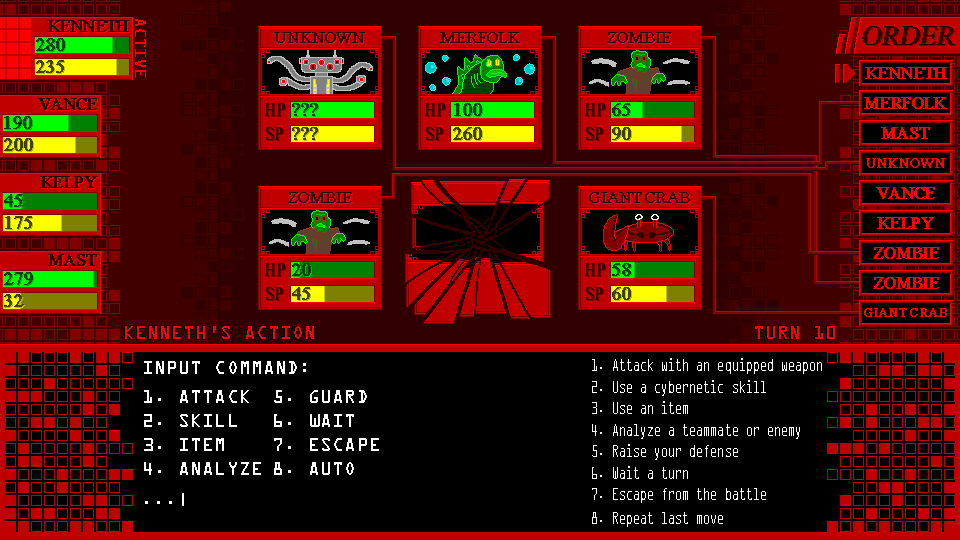
\includegraphics[height=281.25px, width=500px]{Mockups/CYBERNUKE_COMBAT_MOCKUP.png}
\caption{CYBERNUKE Combat Screen Mockup}
\label{combat_mockup}
\end{figure}

\subsection{Interface Mockups}
At first, this will largely be completely made up, as you get further along in your project, and closer to a final product, this will typically become simple screenshots of your running application.

In this subsection, you will be showing what the screen should look like as the user moves through various use cases (make sure to tie the interface mockups back to the specific use cases they illustrate).



% PROJECT TIMELINE ********************************************************************* %
\section{Project Timeline}
Go back to your notes and look up a typical project development life cycle for the Waterfall approach.  How will you follow this life cycle over the remainder of this semester?  This will usually involve a chart showing your proposed timeline, with specific milestones plotted out.  Make sure you have deliverable dates from the course schedule listed, with a plan to meet them (NOTE: these are generally optimistic deadlines).



% PROJECT STRUCTURE ******************************************************************** %
\section{Project Structure}
At first, this will be a little empty (it will need to be filled in by the time you turn in your final report).  This is your chance to discuss all of your design decisions (consider this the README's big brother).

\subsection{UML Outline}
Show the full structure of your program.  Make sure to keep on updating this section as your project evolves (you often start out with one plan, but end up modifying things as you move along).  As a note, while Dia fails miserably at generating pdfs (probably my fault), I have had much success with png files.  Make sure to wrap your images in a \texttt{figure} environment, and to reference with the \texttt{ref} command.  For example, see Figure \ref{main_menu_mockup}.

\begin{figure}[ht!]
\centering
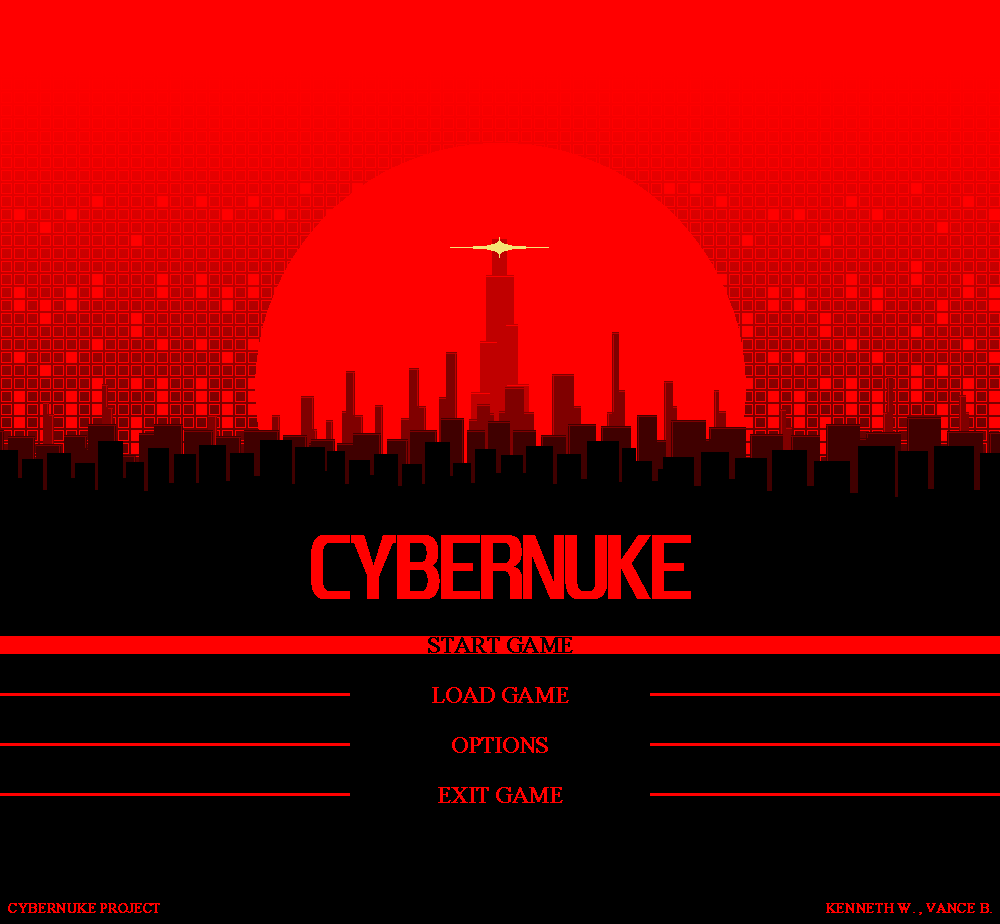
\includegraphics[height=462px, width=500px]{Mockups/CYBERNUKE_MAIN_MENU_2.png}
\caption{CYBERNUKE Main Menu Screen Mockup}
\label{main_menu_mockup}
\end{figure}


\subsection{Design Patterns Used}
Make sure to actually use at least 2 design patterns from this class.  This is not normally part of such documentation, but largely just specific to this class -- I want to see you use the patterns!



% RESULTS ****************************************************************************** %
\section{Results}
This section will start out a little vague, but it should grow as your project evolves.  With each deliverable you hand in, give me a final summary of where your project stands.  By the end, this should be a reflective section discussing how many of your original goals you managed to attain/how many desired use cases you implemented/how many extra features you added.

\subsection{Future Work}
Where are you going next with your project?
For early deliverables, what are your next steps?  (HINT: you will typically want to look back at your timeline and evaluate: did you meet your expected goals?  Are you ahead of schedule?  Did you decide to shift gears and implement a new feature?)
By the end, what do you plan on doing with this project?  Will you try to sell it?  Set it on fire?  Link to it on your resume and forget it exists?


%How to cite: (stuff that needs citation)\cite{IEEEhowto:kopka}.
% BIBLIOGRAPHY ************************************************************************* %
\bibliographystyle{IEEEtran}
\bibliography{./reference}

\begin{thebibliography}{1}

\bibitem{IEEEhowto:cyberpunk}
Britannica, T. Editors of Encyclopaedia. \emph{"cyberpunk."} Encyclopedia Britannica, 1999. https://www.britannica.com/art/cyberpunk.

\bibitem{IEEEhowto:roguelite_1}
Wiktionary. \emph{"roguelite"}
https://en.wiktionary.org/wiki/rogue-lite

\bibitem{IEEEhowto:roguelite_2}
whatNerd, Joel Lee. \emph{"What’s a Roguelike vs. Roguelite? Is the Difference Really That Important?"} whatNerd, 2021. https://whatnerd.com/what-is-a-roguelike-roguelite-difference/.

\end{thebibliography}

% END ********************************************************************************** %
\end{document}


